\documentclass{article}
\usepackage[utf8]{inputenc}
\usepackage[margin=1in]{geometry}
\usepackage{graphicx}
\usepackage{amsmath,amscd}
\usepackage{amssymb}
\usepackage{amsthm}
\usepackage{mathptmx}

\author{Sipu Ruan, Qianli Ma, Gregory S. Chirikjian}
\title{Allowable Motion of Containment for Ellipsoid}

\begin{document}

\maketitle

\section{Mathematical Preliminary}
\subsection{General settings}
Let ${\bf a}=[a_1, a_2, ..., a_n]^T \in \mathbb{R}^n$ denotes the semi-axis of the smaller $n$ dimensional ellipsoid $E_a$, and so the semi-axis of bigger ellipse $E_b$ can be defined as ${\bf b}=[b_1,b_2, ..., b_n]^T=(1+\epsilon){\bf a}$, where $\epsilon \in (0,1]$ is the ``enlarging factor''. The $n$ dimensional ellipsoid can be implicitly represented by
\begin{equation}
({\bf x-t})^T A ({\bf x-t}) = 1 
\end{equation}
where ${\bf t} \in \mathbb{R}^n$ is the center position of the ellipsoid, and the eigenvalue decomposition of $A = R \Lambda^{-2} R^T$ gives a diagonal matrix $\Lambda$ whose diagonal entries are the lengths of semi-axis, and a rotation matrix $R \in SO(n)$ that represents the orientation of the ellipsoid. And the explicit expression can then be defined as
\begin{equation}
{\bf x} = R \Lambda {\bf u} + {\bf t}
\end{equation}
where ${\bf u}$ is the explicit expression of an $n$ dimensional unit sphere with the following properties
\begin{equation}
0 \leq {\bf u}_i^2 \leq 1; -1/2 \leq {\bf u}_i {\bf u}_j \leq 1/2 (i\neq j).
\end{equation}

\subsection{Pose Change Group and its Lie Algebra}
The rotation matrix and position vector introduced above forms a group called ``Pose Change Group'' (PCG) as $(R,{\bf t}) \in PCG(n)$. The corresponding Lie Algebra can be obtained by logarithm map as $[{\bf \omega}^T, {\bf t}^T]^T \in \mathbb{R}^{n(n+1)/2}$, where ${\bf \omega}=\log^\vee(R)$ is the vector form of the matrix logarithm of the rotation matrix, which is a skew-symmetric matrix. The Lie Algebra can be transformed back to the Lie Group by exponential map, i.e. $(\exp(\hat{\bf \omega}), {\bf t}) \in PCG(n)$.

\subsection{Algebraic condition of containment}
By substituting the explicit expression of the moving smaller ellipsoid $E_a$ into the implicit expression of the larger ellipsoid $E_b$ that is fixed at the origin with orientation being identity, the algebraic condition for $E_a$ to move inside of $E_b$ without collision can be written as
\begin{equation}
\label{eq:condition_origin}
(R_a \Lambda({\bf a}) {\bf u} + {\bf t}_a)^T \Lambda^2({\bf b}) (R_a \Lambda({\bf a}) {\bf u} + {\bf t}_a) \leq 1.
\end{equation}

Once we enforce $\epsilon$ to be small, the rotation part calculated by exponential map can be approximated by the first order Taylor series as
\begin{equation}
\label{eq:rotation_approx}
R_a = \exp(\hat{\omega}_a) \approx \mathbb{I} + \hat{\omega}_a.
\end{equation}
Substituting Eq.~\ref{eq:rotation_approx} into Eq.~\ref{eq:condition_origin} and grouping parameters (${\bf u}$) and variables (${\bf \omega}$) gives the first-order approximation of the algebraic condition of containment as
\begin{equation}
C({\bf \omega}) = {\bf \omega}^T H({\bf u}) {\bf \omega} + {\bf h}^T({\bf u}) {\bf \omega} + c({\bf u}) \leq 1.
\end{equation}

\section{Closed-form Lower Bound of the Configuration Space}
%%%%%%%%%%%%%%%%%%%%%%%%%%%%%%

\section{Configuration Space that has Larger Volume Generated via Convex Optimization}
By observation from the sample-based KC, surfaces between 3 different extreme points which seems flat forms a polyhedron-shaped c-space. This gives an intuition to construct the motion c-space with a larger volume fitting a polyhedron to the samples. We first seek to find the extreme points that represent the polyhedron as follows.

\subsection{Finding extreme vertices that represent the polyhedron}
There are 2 cases to be considered when searching for the vertices of the polyhedron: (1) extreme points that lies on each axis of the c-space; (2) points that are farthest to the origin.

Extreme points in each axis can be simply found by fixing the other axis lengths to zero. Since in each axis, there are 2 extreme points (positive and negative), we get $2n$ vertices for the first case. For the vertices that are farthest to the origin, we seek to maximize the distance function to origin, i,e, $f = {\bf z}^T {\bf z}$. Further, the constraint for ${\bf z}$ is that the rotational and translational parts should satisfy the algebraic condition that the smaller ellipse $E_a$ must move inside the larger one $E_b$ without collision as
\begin{equation}
(R(\theta) \Lambda({\bf a}) {\bf u} + {\bf t})^T \Lambda^{-2}({\bf b}) (R(\theta) \Lambda({\bf a}) {\bf u} + {\bf t}) \leq 1.
\end{equation}
Regrouping the terms of the first-order approximation of the above inequality gives the constraint for ${\bf z}$ as 
\begin{equation}
C({\bf z}) = {\bf z}^T H({\bf u}) {\bf z} + {\bf h}({\bf u})^T {\bf z} + c({\bf u}) \leq 1.
\end{equation}

Such constraint is a family of inequality constraints where ${\bf u}_i$ represents the $i$-th point on the boundary of a unit sphere. If we treat ${\bf z}$ as unknown variable and ${\bf u}$ as a group of known parameters, finding the maximum distance can be formed as an optimization problem as follows

\begin{equation}
\begin{aligned}
& {\bf z}_{extreme} = \arg\max {\bf z}^T {\bf z} \\
\text{{\bf s.t.   }} & C_i({\bf z}) = {\bf z}^T H({\bf u}_i) {\bf z} + {\bf h}({\bf u}_i)^T {\bf z} + c({\bf u}_i) \leq 1 & (i=0,...,m)\\
\end{aligned}
\end{equation}
where, $m$ is the number of discretized points on the boundary of the unit sphere.

Since the objective function is quadratic, the solutions for each variable have 2 possibilities, so the total number of solutions can be up to 8. However, not all of those possibilities are feasible solutions, meaning we have to validate them by substituting back to the constraint inequalities. Interestingly, after some numerical tests, there are only 4 of them that are feasible, i.e. for each fixed $x,y$ pair, there is only one corresponding $\theta$ that the smaller ellipse can stay inside the large one without collision. Fig \ref{polyfit_cspace} and \ref{polyfit} show the resulting c-space polyhedron and the corresponding scenarios in euclidean space.

At this time, we get totally 10 extreme vertices to construct the ``c-space motion polyhedron''. By saying ``polyhedron'', we should prove that the surfaces we observed is truly flat, in other word, points on the straight line connecting two vertices all represent safe configurations. This observation becomes obvious if we could firstly show that the constraint functions are convex.

\subsection{Show that the c-space points inside the convex hull of the extreme vertices are safe configurations}
We have the following equivalent claim: the c-space points that lies on the line segment connecting any two extreme points also satisfy the conditions $C({\bf z}) = {\bf z}^T H({\bf u}) {\bf z} + {\bf h}({\bf u})^T {\bf z} + c({\bf u}) \leq 1$ for all ${\bf u} \in \mathcal{B}(1)$.

%%% Proof of claim %%%%
\begin{proof}
	From the condition we could also claim that among all ${\bf u}$,
	\begin{equation}
	\label{proof_convex}
	\max C_i({\bf z}) = \max {\bf z}^T H({\bf u}_i) {\bf z} + {\bf h}({\bf u}_i)^T {\bf z} + c({\bf u}_i) \leq 1
	\end{equation}
	
	Then we could further prove that ``given any two extreme points ${\bf z}_1, {\bf z}_2$ satisfying \eqref{proof_convex}, the points on line segment between these two points also satisfy \eqref{proof_convex}''. The proof can be achieved by showing $\max C_i({\bf z})$ is convex.
	
	For any fixed ${\bf u}_i$, we seek to prove, at first, that the function $C_i({\bf z})$ is convex, which is to show that, given ${\bf z}_1, {\bf z}_2$
	
	\begin{equation}
	\label{proof_convex_ineq}
	C_i(\alpha {\bf z}_1 + (1-\alpha) {\bf z}_2) \leq \alpha C_i({\bf z}_1) + (1-\alpha) C_i({\bf z}_2),  \forall  \alpha \in [0,1]
	\end{equation}
	
	Expanding both sides and moving right-hand side to the left gives
	
	\begin{equation}
	\label{proof_convex_each}
	\begin{aligned}
	& [LHS]-[RHS] \\
	=& [(\alpha {\bf z}_1 + (1-\alpha) {\bf z}_2)^T H({\bf u}_i) (\alpha {\bf z}_1 + (1-\alpha) {\bf z}_2) + {\bf h}({\bf u}_i)^T (\alpha {\bf z}_1 + (1-\alpha) {\bf z}_2) + c({\bf u}_i)]\\
	& - [\alpha ({\bf z}_1^T H({\bf u}_i) {\bf z}_1 + {\bf h}({\bf u}_i)^T {\bf z}_1 + c({\bf u}_i)) + (1-\alpha)({\bf z}_2^T H({\bf u}_i) {\bf z}_2 + {\bf h}({\bf u}_i)^T {\bf z}_2 + c({\bf u}_i))] \\
	=& -\alpha(1-\alpha) [({\bf z}_1 - {\bf z}_2)^T H({\bf u}_i) ({\bf z}_1 - {\bf z}_2)]
	\end{aligned}
	\end{equation}
	
	The above expression satisfies the inequality $[LHS]-[RHS] \leq 0$ if and only if $({\bf z}_1 - {\bf z}_2)^T H({\bf u}_i) ({\bf z}_1 - {\bf z}_2) \geq 0$, or equivalently, $H({\bf u}_i)$ is symmetric positive semi-definite, which can be showed by expanding the original expression of the condition to the 1st-order approximation.
	
	Since ${\bf z} = [{\bf r}^T, {\bf t}^T]^T$, only the quadratic terms with respect to both ${\bf r}$ and ${\bf t}$ from the 1st-order approximation will contribute to the calculation of ${\bf z}^T H({\bf u}_i) {\bf z}$ for any ${\bf z}$. Thus, we have, $\forall {\bf z} \in \mathfrak{R}^{\frac{n(n+1)}{2}}$
	
	\begin{equation}
	\label{proof_convex_psd}
	{\bf z}^T H({\bf u}_i) {\bf z} = (S({\bf r}) \Lambda({\bf a}) {\bf u} + {\bf t})^T \Lambda^{-2}({\bf b}) (S({\bf r}) \Lambda({\bf a}) {\bf u} + {\bf t})
	\end{equation}
	
	Since $\Lambda^{-2}({\bf b})$ is diagonal with non-negative entries on diagonal, \eqref{proof_convex_psd} $\geq 0$, which means that $H({\bf u}_i)$ is symmetric positive semi-definite. Hence we showed the inequality condition for \eqref{proof_convex_each}, from which we conclude that each condition function $C_i({\bf z})$ is convex.
	
	Next, we continue the proof by showing that the maximum of a family of convex functions is also convex. Since $C_i({\bf z})$ is convex, then taking maximum for both sides of \eqref{proof_convex_ineq} gives
	
	\begin{equation}
	\begin{aligned}
	\max C_i(\alpha {\bf z}_1 + (1-\alpha) {\bf z}_2) &\leq \max [\alpha C_i({\bf z}_1) + (1-\alpha) C_i({\bf z}_2)],  \forall  \alpha \in [0,1]\\
	&\leq \max \alpha C_i({\bf z}_1) + \max (1-\alpha) C_i({\bf z}_2),  \forall  \alpha \in [0,1] \\
	\end{aligned}
	\end{equation}
	
	Thus $\max C_i({\bf z})$ is convex. And we can conclude that if for two extreme points ${\bf z}_1, {\bf z}_2$, $\max C_i({\bf z}_j) \leq 1, j=1,2$ are hold, then for points on the line segment between them, $\alpha {\bf z}_1 + (1-\alpha) {\bf z}_2, \forall \alpha \in [0,1]$, $\max C_i(\alpha {\bf z}_1 + (1-\alpha) {\bf z}_2) \leq \alpha \max C_i({\bf z}_1) + (1-\alpha) \max C_i({\bf z}_2) \leq 1$ is also satisfied. 
\end{proof}
%%%%%%%%%%
%%%%%%%%%%%%%%%%%%%%%%%%%%%%%%

\section{Examples in SE(2)}
\subsection{Largest angle that the smaller ellipse can rotate}
The maximum angle that the smaller ellipse can rotate comes when the center point is fixed in the origin. And the angle can be found in closed-form as follows.

We use the parametric forms for the two ellipses,
\begin{equation}
\begin{aligned}
{\bf u}_a = \left( 
\begin{aligned}
a_1 \cos \theta_a\\
a_2 \cos \theta_a
\end{aligned}
\right) &&
{\bf u}_b = \left( 
\begin{aligned}
b_1 \cos \theta_b\\
b_2 \cos \theta_b
\end{aligned}
\right)
\end{aligned}
\end{equation}

and the rotation of $E_a$ can be written as,
\begin{equation}
R(\phi) = \left(
\begin{aligned}
\cos\phi && -\sin\phi\\
\sin\phi && \cos\phi
\end{aligned}\right)
\end{equation}
where $\phi$ is the rotational angle of $E_a$.

Assume that the bigger ellipse $E_b$ is fixed with the world frame, with the center in the origin, and the larger semi-axis is aligned with x-axis. Then the points on the boundary of $E_b$ as seen in the world frame is exactly ${\bf u}_b$. Since $E_a$ only rotates around the origin, the points on its boundary as seen in the world frame should be $R(\phi) {\bf u}_a$.

The intersecting point of the two ellipses can be obtained by enforcing the two parametric equations as seen in the world frame to be equal as,
\begin{equation}
\begin{aligned}
& {\bf u}_b = R(\phi) {\bf u}_a \\
\iff & \left\{
\begin{aligned}
b_1 \cos\theta_b = a_1\cos\phi \cos\theta_a - a_2\sin\phi \sin\theta_a\\
b_2 \sin\theta_b = a_1\sin\phi \cos\theta_a + a_2\cos\phi \sin\theta_a
\end{aligned}
\right.\\
\end{aligned}
\end{equation}
Substituting $a_1 = \alpha a_2, b_1 = (1+\epsilon)a_1, b_2 = (1+\epsilon)a_2$, and observing the fact that $\theta_b = \phi + \theta_a$ (rotational angle transformation from local frame to world frame of $E_a$) gives,
\begin{equation}
\begin{aligned}
& \left\{
\begin{aligned}
\alpha a_2 (1+\epsilon) \cos(\theta_a + \phi) = \alpha a_2 \cos\phi \cos\theta_a - a_2\sin\phi \sin\theta_a\\
a_2 (1+\epsilon) \sin(\theta_a + \phi) = \alpha a_2 \sin\phi \cos\theta_a + a_2\cos\phi \sin\theta_a
\end{aligned}
\right. \\
\iff & 
\left\{
\begin{aligned}
\alpha \epsilon \cos\theta_a \cos\phi = (\alpha(1+\epsilon) - 1) \sin\theta_a \sin\phi \\
\epsilon \sin\theta_a \cos\phi = (\alpha - \epsilon - 1) \cos\theta_a \sin\phi \\
\end{aligned}
\right. \\
\end{aligned}
\end{equation}
Since always $a_2 < b_2$, the points on smaller semi-axis of the smaller ellipse will be always inside the bigger ellipse, so when we consider the case of intersecting, $\theta_a \neq \pi/2$, or $3\pi/2$, or $\cos\theta_a \neq 0$. Further, One sufficient condition when two ellipses intersect should be $a_1 \geq b_2$, or $\alpha \geq 1+\epsilon$, and the equal sign occurs only when $\phi = \pi/2, 3\pi/2$ and $\theta_a = 0, \pi$, or $\cos\phi = 0$ and $\sin\theta_a = 0$.

So, for general cases, we could rearrange the above system of equations as,
\begin{equation}
\left\{
\begin{aligned}
\frac{\alpha \epsilon}{(\alpha(1+\epsilon)-1)} = \tan\theta_a \tan\phi \\
\frac{\epsilon}{(\alpha - \epsilon - 1)} \tan\theta_a = \tan\phi
\end{aligned}
\right.
\end{equation}
Since $b_1 \geq a_1$, $\phi \neq 0, \pi$ ($\tan\phi \neq 0$) when two ellipses intersect, then we could get,
\begin{equation}
\begin{aligned}
& \frac{\alpha \epsilon}{(\alpha(1+\epsilon)-1) \tan\phi} = \frac{(\alpha - \epsilon - 1) \tan\phi}{\epsilon}\\
\Rightarrow & \tan^2\phi = \frac{\alpha \epsilon^2}{(\alpha(1+\epsilon)-1)(\alpha - \epsilon - 1)}
\end{aligned}
\end{equation}
Solving for $\phi$ gives,
\begin{equation}
\phi = \arctan (\pm \epsilon \sqrt[]{\frac{\alpha}{(\alpha(1+\epsilon)-1)(\alpha - \epsilon - 1)}})
\end{equation}

Figures \ref{diff-alpha} and \ref{diff-epi} show the numerical experiments to verify the result, with different $\alpha$ and $\epsilon$ values respectively.

\begin{figure}
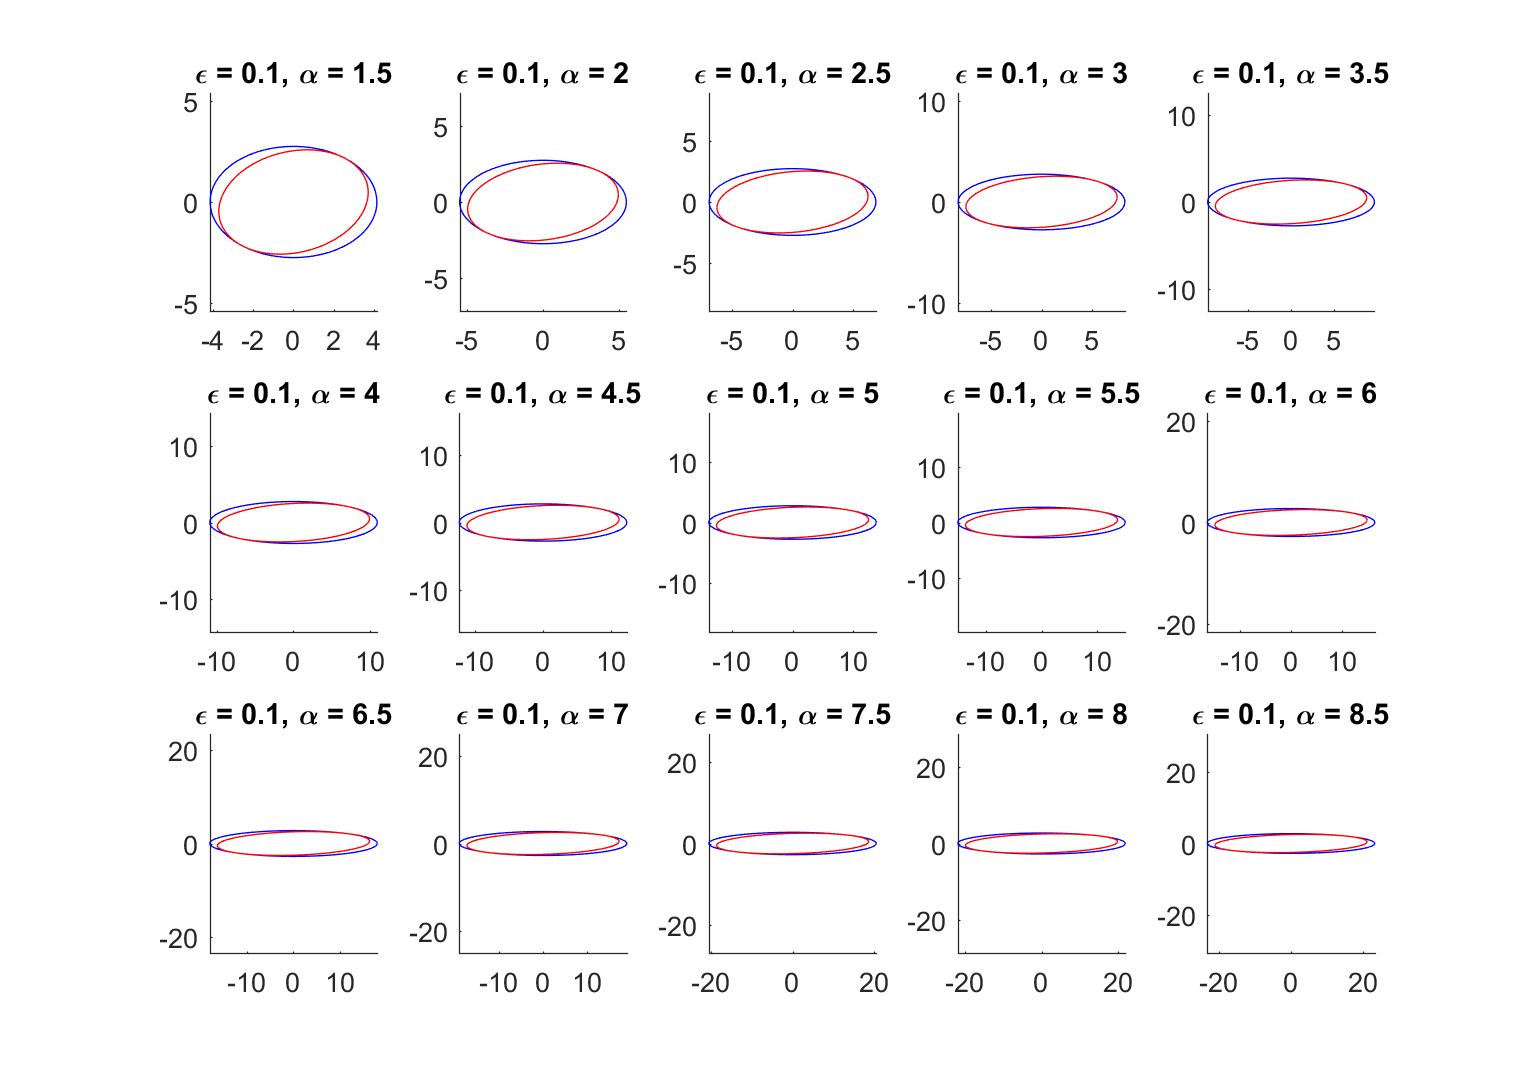
\includegraphics[scale = 0.17]{fig/closed-form_maxAngle-test_alpha.png}
\caption{Test with different values of aspect ratio $\alpha$, fixed $\epsilon = 0.1$}
\label{diff-alpha}
\end{figure}

\begin{figure}
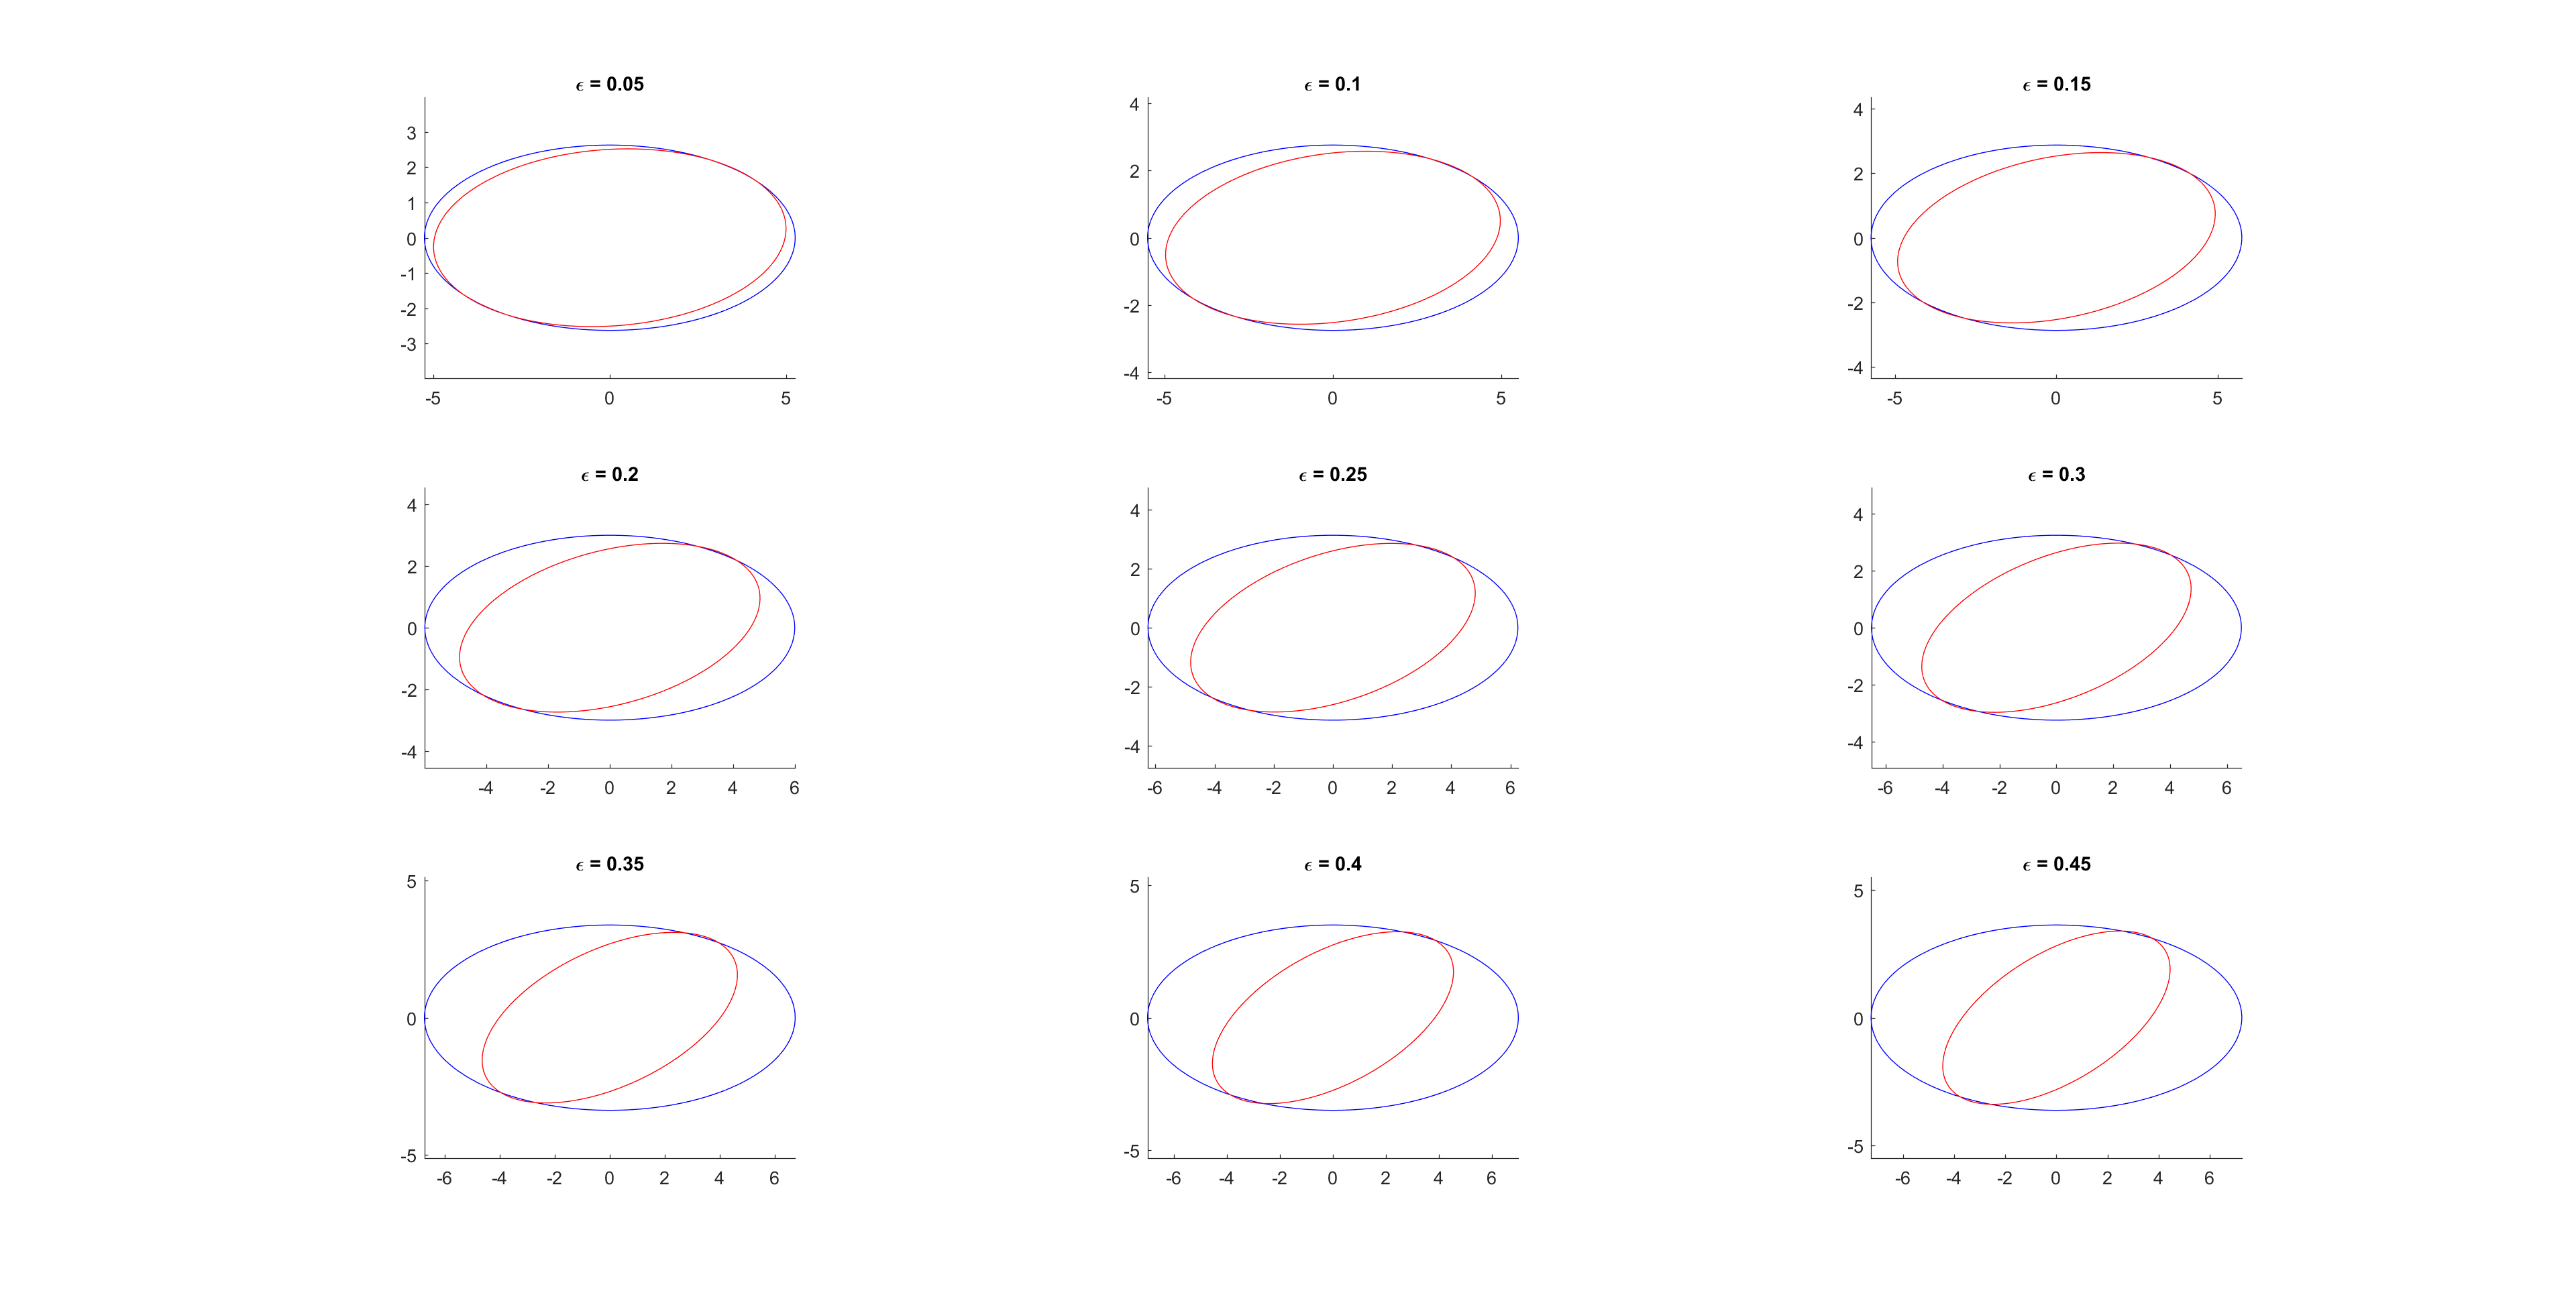
\includegraphics[scale = 0.17]{fig/closed-form_maxAngle-test_epsilon.png}
\caption{Test with different values of explode factor $\epsilon$, fixed $\alpha = 2$}
\label{diff-epi}
\end{figure}
%%%%%%%%%%%%%%%%%%%%%%%%%%%%%%

\subsection{Results}
Figs \ref{polyfit_cspace_10000samples} and \ref{polyfit_10000samples} show the numerical results of randomly sampled configurations of smaller ellipses that verify the above claim. The ellipse whose configuration point is inside the c-space polyhedron (convex hull of the 10 extreme vertices) lies safely inside the larger one without collision.

\begin{figure}[t]
\centering
\begin{minipage}[b]{0.4\textwidth}
	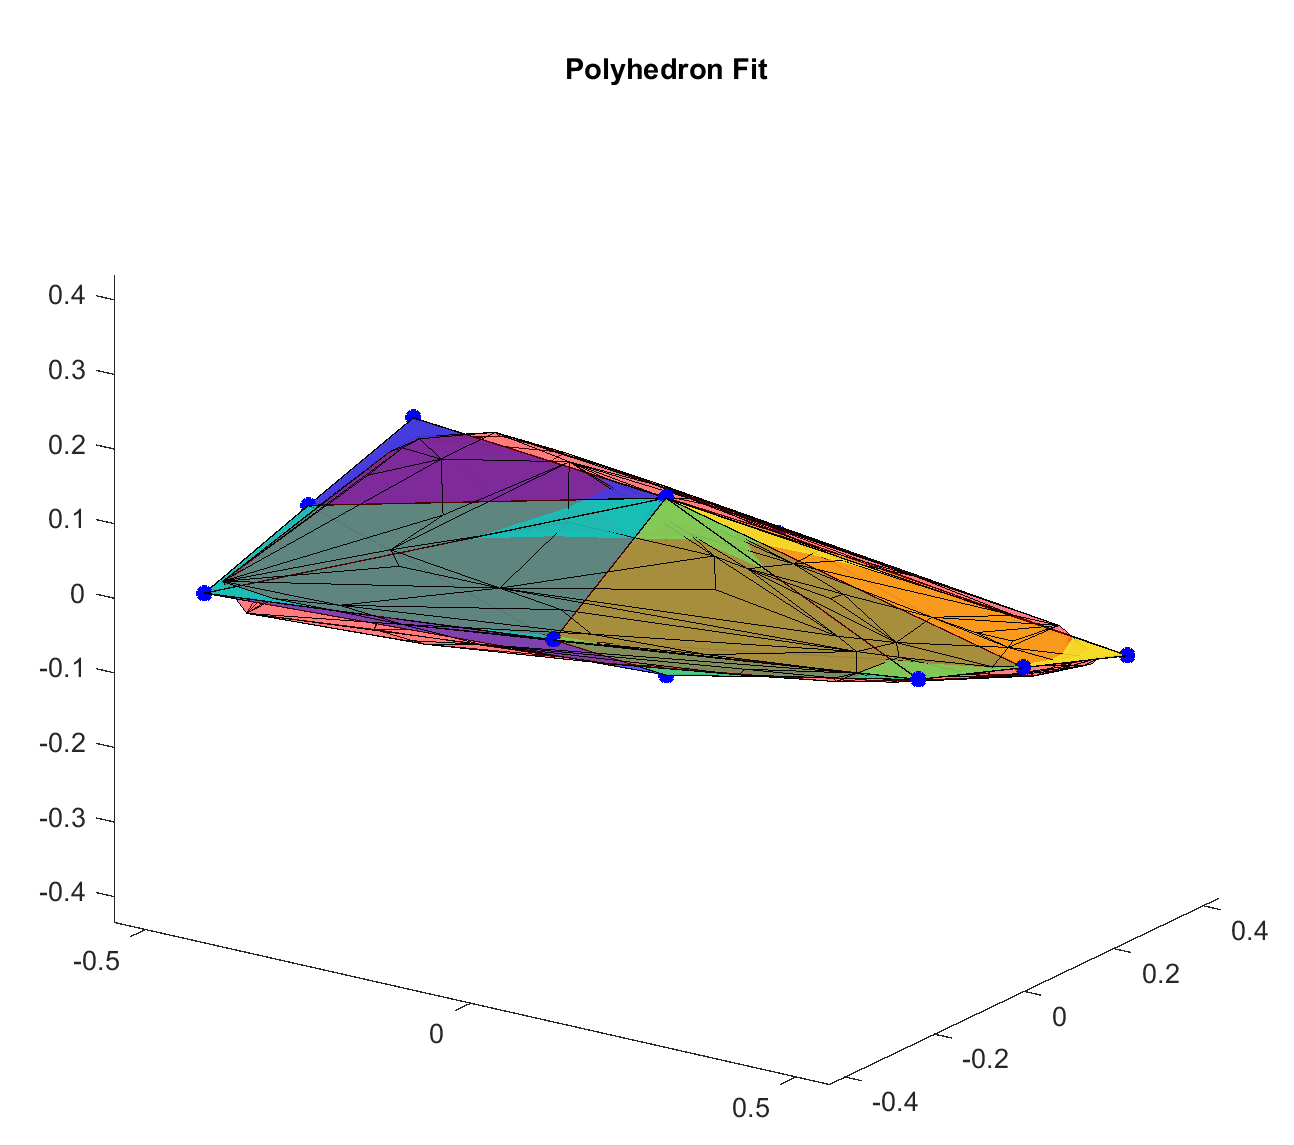
\includegraphics[scale = 0.2]{fig/c-space-polyhedron-fit.png}
	\caption{Heuristic fit as polyhedron represented by 10 extreme vertices, C-space}
	\label{polyfit_cspace}
	\end{minipage}
	\hfill
	\begin{minipage}[b]{0.4\textwidth}
		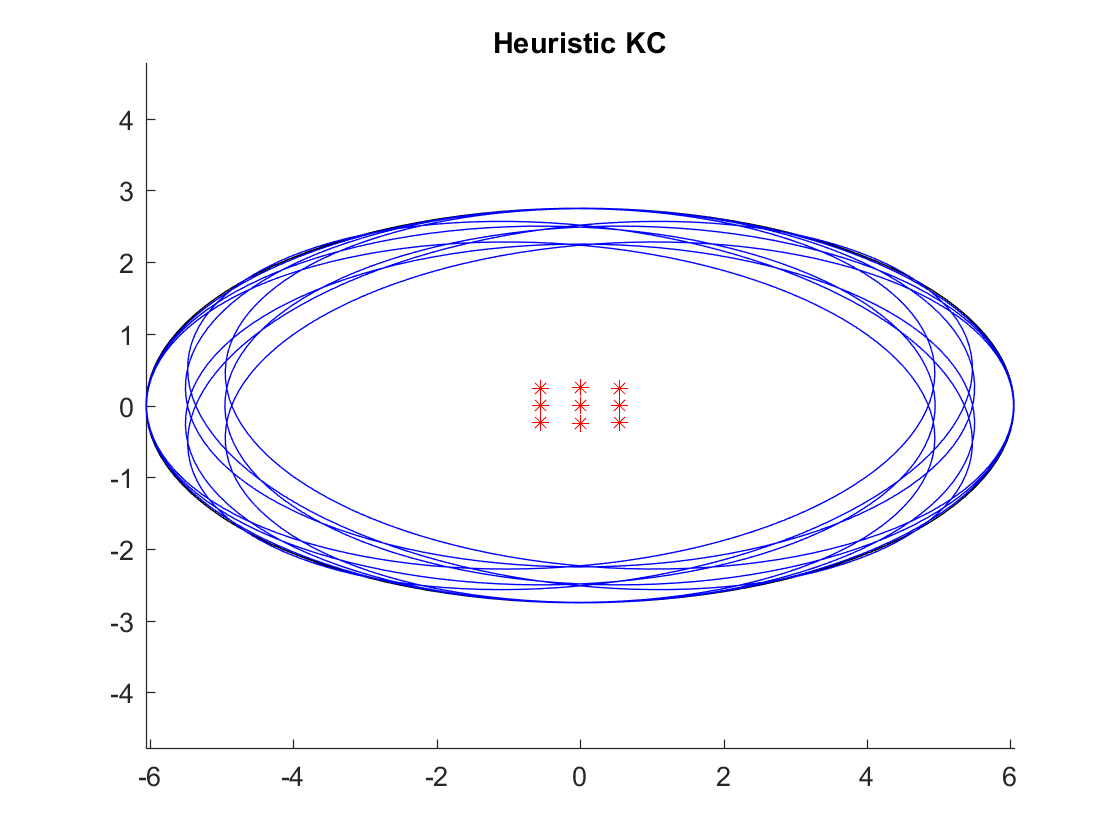
\includegraphics[scale = 0.25]{fig/ellipses-polyhedron-fit.png}
		\caption{Heuristic fit as polyhedron represented by 10 extreme vertices}
		\label{polyfit}
		\end{minipage}
\end{figure}

\begin{figure}[t]
	\centering
	\begin{minipage}[b]{0.4\textwidth}
		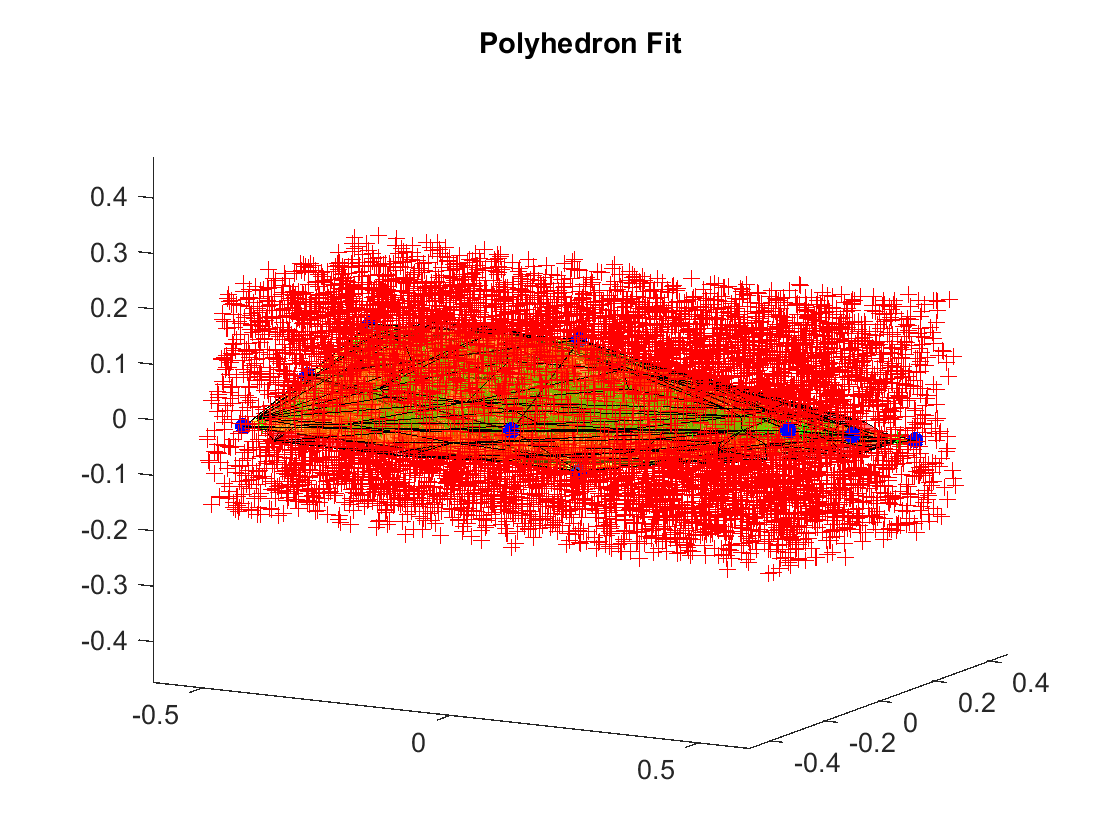
\includegraphics[scale = 0.2]{fig/c-space-polyhedron-fit-with-testPnts10000.png}
		\caption{C-space polyhedron fit with samples. Red: outside the convex hull; green: inside the convex hull}
		\label{polyfit_cspace_10000samples}
	\end{minipage}
	\hfill
	\begin{minipage}[b]{0.4\textwidth}
		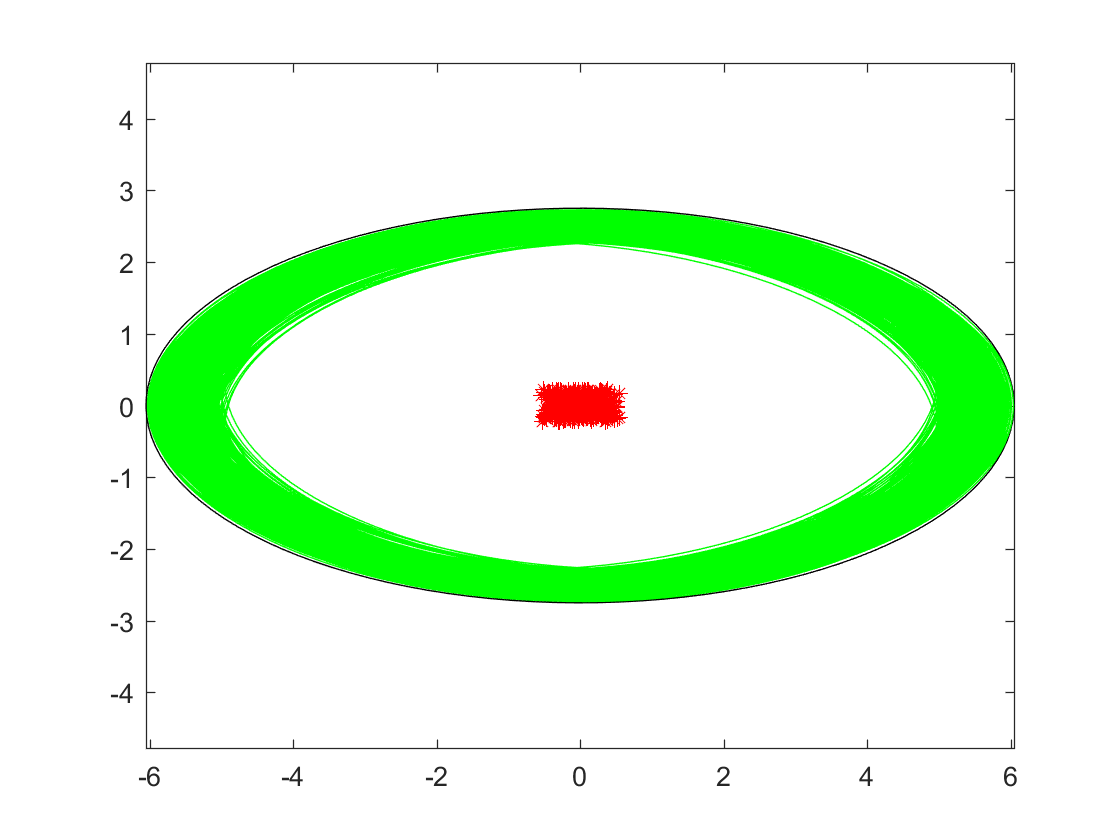
\includegraphics[scale = 0.25]{fig/ellipses-polyhedron-fit-with-testPnts10000.png}
		\caption{Smaller ellipses that lies safely inside the larger ellipse.}
		\label{polyfit_10000samples}
	\end{minipage}
\end{figure}
%%%%%%%%%%%%%%%%%%%%%%%%%%%%%%
\end{document}
